% !TEX root = ../ac_paper.tex

\section{Language Modeling}

\fixme{Can we model the language of balanced presentations of the trivial group in general, somehow? What can one hope to learn from that?}

\fixme{Not very happy with the results of this section.}

\fixme{Can we conclude from this section or from this paper somehow that $n$ as compared to total length is a better metric for hardness of examples from the Miller-Schupp series?}

\fixme{Within examples of the same value of $n$, what distinguishes between hard vs easy problems? Is it length of the word $w$? Or is it some other property? Perhaps the count of $x$'s. Perhaps the count of $y$'s.}

\fixme{One thing that t-SNE projections show is that for most values of $n$, there are two clusters: one containing a mix of solved and unsolved examples, and another containing only the unsolved examples. 1). Why is that? 2). Can we measure what distinguishes the two clusters? Is it length of $w$, is it the number of $x$'s vs $y$'s, or is it something else? 3). Can we say that the unsolved presentations in the former cluster are more likely to be solvable than the problems in the latter cluster?}

\fixme{It seems that the goal for us is not to model the language as such, but to find an embedding of the examples, and see if this embedding space, also known as 'latent space' contains any useful information about the question of hardness of examples.}

\fixme{The clustering with $n$ is not a miracle. That's just a consequence of our tokenization. The clustering of hard vs easy examples within each $n$, that's more interesting.}

The probability of a document 

\[
p(t_1 \cdots t_{n_c}) = \prod\limits_{i=1}^{n_c} p (t_{i} \mid t_{1} \cdots t_{i-1}) 
\]

$p (t_{n} \mid t_{1} \cdots t_{n-1}) $ is the $n$-gram probability distribution of text. Decoder-only transformer models learn this probability distribution from a dataset of text. 
\newline

Perplexity: https://huggingface.co/docs/transformers/en/perplexity

An advantage of using transformers or neural networks is that you can also find an embedding of words/sentences \cite{Bengio:2003}. The similarity of texts actually reflects in the geometry of the embedding vectors: similar texts are closer to each other when measured by cosine similarity. [

Here, we model the langauge of balanced presentations of the trivial group with two generators and ask if the geometry of embedding vectors reflects any structure of 

In section 4.1, we give a review of decoder-only transformers; in section 4.2, we discuss the dataset used to train the model; and in section 4.3, we present our results. 

\footnote{For a review of decoder-only transformer models and Large Language Models aimed at physicists and mathematicians, see \cite{douglas2023large,}.}

\footnote{\fixme{What is the correct reference for analyzing embeddings through cosine simiarity between vectors?}}

Original attention paper: \cite{vaswani2023attention}.

Previously, encoder-only architectures were used in \cite{gukov2020learning} for the unknot decision problem. 


\subsection{Transformers: a review}

Here, we give a short review of the architecture of a decoder-only transformer. Given an input sequence $t_1, t_2, \cdots, t_{n_c}$, a decoder-only transformer predicts the probability distribution over the vocabulary, i.e. it predicts $p(t \mid t_1, t_2, \cdots, t_{n_c})$ for each $t$ in the vocabulary. We will denote the size of the vocabulary as $n_v$. Each elements of the vocabulary is often referred to as a `token'. The probability distribution for the $(n_c+1)$-st token is predicted by applying the following sequence of functions to the input sequence.

The presentation given here is slightly different from the original presentation. We follow \cite{elhage2021mathematical}.

We start with encoding our input sequence into a matrix $T \in \R^{n_c \times n_v}$, \fixme{Convert $t_i$ into a number first.}
\footnote{Each row of $t$ is often referred to as a `one-hot encoded vector'.}
\[
T_{ij} = \delta_{i t_i}
\]
and embed each token into a $\dm$-dimensional space with the help of an embedding matrix $W_E \in \R^{\dm \times n_v}$,
\[
x_0 = (\mathbb{1} \otimes W_E) T
\]

\fixme{positional encoding} $W_P$ should be a matrix of shape ?

For an $L$-layer transformer, we alternate between applying a ``multi-head attention" transformation and an ``MLP-layer" transformation as follows. 
\[
x_{2i+1} = x_{2i} + \sum_{h \in H_j} h(\mathbb{1} \otimes \LN(x_{2i})) 
\]
\[
x_{2i + 2} = x_{2i + 1} + \FFN(\mathbb{1} \otimes \LN(x_{2i + 1}))
\]
where $i=0, \cdots, L-1$. Note that $x_j \in \R^{\nc \times \dm}$ for all $j = 0, 1, \cdots, 2L$, and a row of $x_j$ is seen as a vector in $\R^{\dm}$ associated to a token $t_i$ in the input text. $\LN$ is the ``Layer Normalization" operation \fixme{Include citation} 


that we will describe below. The multi-head attention transformation $\sum_{h \in H_j} h$ is a sum over various ``attention-heads", with each attention-head function $h$ acting as follows.
\[
h(x) = (A \otimes W_O W_V) x
\]
Here, $A \in \R^{n_c \times n_c}$ is defined as
\[
A = \softmax(x^T W_Q^T W_K x)
\] 
$W_O \in \R^{\dm \times \dhead}$, and 
The number of attention heads is a hyperparameter of the architecture.


Apply LN right before the unembed operation. 

How does unembed work? 

Why do we learn $W_O$ and $W_V$ separately and $W_Q$ and $W_K$ separately? Why don't we put them together into one? Does it have to do with $W_O W_V$ and $W_{Q^T} W_K$ being low-rank? Why do $W_O W_V$ and $W_{Q^T} W_K$ have to be low-rank and is it hard to learn low-rank matrices directly? 

$W_Q$, $W_K$ and $W_V$ project from a higher dimensional space $\R^\dm$ to a lower-dimensional space $\R^\dhead$, therefore, they must have large null spaces. (On the other hand, $W_O$ projects from the lower-dimensional space $\R^\dhead$ to $\R^\dm$.) The products $W_O W_V$ and  $W_Q^T W_K$ might be low-rank because of this reason.

Should $\R^{\dhead}$ be seen as a subspace of $\R^{\dm}$ or should it be seen as an independent space of its own? I don't know if this is actually a precise question. 

Right below I mention that $W_O W_V$ acts on $x$, I should mention why we train 
Include Layer Normalizations. 
Include reference to Layer Normalization. 

Cross entropy.

Why Layer Normalization and not batch normalization? https://stats.stackexchange.com/questions/474440/why-do-transformers-use-layer-norm-instead-of-batch-norm

What does it mean to read and write from the residual stream? 

What does LayerNorm actually do? Make things zero/small/large, etc. Consider a model where layernorm is used versus not. 

This article has a section on "Linearizing LayerNorm aka Ignoring LayerNorm aka Fixing LayerNorm: ". It will be useful. Don't get scared by the size of the page. Most of it is stuff you already know.

https://www.neelnanda.io/mechanistic-interpretability/glossary

Also Chris Olah says the following thing on the link below. Don't worry about reading the rest of that page.

"LayerNorm in transformers is slightly different from what you describe. There are no interactions between tokens. This is actually the reason LayerNorm is preferred: in autoregressive transformers, one needs to be paranoid about avoiding information leakage from future tokens, and normalization across tokens becomes very complicated as a result, leading to a preference for normalization approaches that are per-token. In any case, there are some minor flow through effects from this to other things you say."

Here is the link: https://www.lesswrong.com/posts/pBFTFMsuaSJX4vCj9/mechanistic-interpretability-for-the-mlp-layers-rough-early

Ah, here is another interesting + useful article on LayerNorm: https://arxiv.org/pdf/2305.02582.pdf


\subsection{Dataset for the GPT model}

We apply sequences of AC moves to the Miller-Schupp series presentations studied in the previous subsection to generate a dataset.
We use Algorithm \autoref{alg:apply_ac_moves} to ensure that the total length of the generated presentations follows roughly a uniform distribution.
(See \autoref{fig:gpt_data}; there, the distribution is roughly uniform with short tails on either side.)
\footnote{Maybe there should be only one histogram in the figure showing combined solved+unsolved statistics.
As it is, I computed separate percentages for each solved/unsolved case.
I should clarify that if I leave the figure as it is.
It is also good to change the total length.
Also change the label of x-axis to something better.}

Algorithm \autoref{alg:apply_ac_moves} generates presentations of increasing lengths in $n$ phases.
In the $i$-th phase, presentations with maximum relator length $l_i$ are generated, where $l_i$ is sampled from a discrete uniform distribution with bounds $l + i l_{\text{inc}} $ and $l + (i+1) l_{\text{inc}}$.
Here, $l$ is the maximum of the lengths of the two relators in the initial Miller-Schupp presentation $R_0$ (and thus the minimum value of maximum relator length in the algorithm), and $l_{\text{inc}}$ is defined in terms of the maximum possible relator length $l_{\text{max}}$ we wish to obtain in the last phase as $l_{\text{inc}} = (l_{\text{max}}-l)/n$.
In the $i$-th phase, $T$ AC moves are applied to a presentation generated in the $(i-1)$-th phase.
In our work, we chose $l_{\text{max}}=128$, $n=128$, $m=12$, and $T=1000$.
\footnote{Specify much earlier in the paper, and here as well, that whenever we apply AC moves, we set a maximum length up to which each relator is allowed to grow.
Any AC move that would result in a presentation of longer relator length acts trivially.
Maybe instead of writing $A \sim \text{AC Moves}$, there should be a notation like $(AC)_l$ when $l$ is specified to be the maximum relator length.}

\begin{algorithm}
	\caption{Generate AC Cousins}\label{alg:apply_ac_moves}
	\begin{algorithmic}
		\Require $R_0$, $l_{\text{max}}$, $n$, $m$, $T$
		\State $L \gets \{ \}$ \Comment{Initiate the list $L$ of all presentations}

		\State $l \gets \max(l_1, l_2)$

		\Comment{Set $l_1$, $l_2$ are the lengths of relators of $R_0$}

		\State $l_{\text{inc}} \gets (l_{\text{max}}-l)/n$

		\Comment{The increment by which the maximum relator length increases in each phase}

		\For {$i = 1, 2, \dots, n$}

		\Comment{Loop over $n$ phases}
		\For {$j = 1, 2, \dots, m$}

		\Comment{Generate $m$ presentations in each phase}
		\State $l_i \sim \mathcal{U}(l + i l_{\text{inc}} , l + (i+1) l_{\text{inc}})$

		\Comment{Set the maximum relator length for $i$-th phase}
		\If{i is 0}
		\State $R \gets R_0$
		\Else
		\State $R \gets L[(i-1) \times m+j]$
		\EndIf

		\Comment{Set $R$ to a presentation of the previous phase if $i > 0$, else set it to the initial presentation $R_0$}


		\For{$k = 1, 2, \dots, T$}

		\Comment{Apply $T$ randomly selected AC-moves}
		\State A $\sim$ AC Moves
		\State $R \gets A \cdot R$

		\EndFor

		\State $L \gets R$

		\Comment{Add the resultant presentation $R$ to $L$}

		\EndFor
		\EndFor
	\end{algorithmic}
\end{algorithm}

The main reason for choosing this algorithm is so that our GPT model sees roughly the same amount of presentations of each length and is, hence, not biased towards shorter or longer presentations.
The final dataset contained 0.8 million (1 million) presentations generated from applying Algorithm \autoref{alg:apply_ac_moves} to BFS-easy (BFS-hard) examples.
Only a small amount (roughly 15 percent) of the original Miller-Schupp presentations remained to be part of this dataset.

\begin{figure}
	\centering
	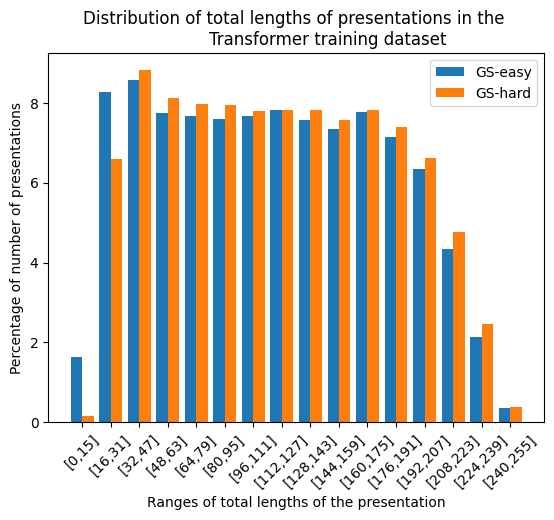
\includegraphics[scale=0.6]{fig/gpt_data_length_distribution.png}
	\caption{Percentage of presentations in various ranges of total lengths.}
	\label{fig:gpt_data}
\end{figure}

The dataset is tokenized by adding two stop tokens that represent the end of two relators of a presentation.
Thus there are six tokens in total: one each for $x$, $y$, $x^{-1}$, and $y^{-1}$ and the two stop tokens.
The tokenized dataset has about 217M tokens, and the distribution of tokens is shown in \autoref{fig:tokens_hist}.
We note that $y$ and $y^{-1}$ appear significantly more often than $x$ and $x^{-1}$ in the unsolved dataset.
This is likely because the BFS-hard examples have higher $n$, and higher $n$ corresponds to more of a presence of $y$ and $y^{-1}$.
Interestingly, this effect remains in the dataset even when we apply thousands of AC moves.
I should investigate this further.

We set aside 10 percent of the data as a validation dataset.

\begin{figure}
	\centering
	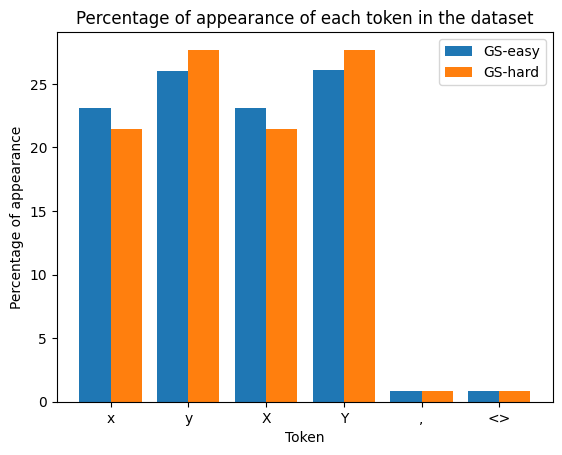
\includegraphics[scale=0.6]{fig/tokens_hist.png}
	\caption{Percentage of appearance of each token in the solved/unsolved datasets.}
	\label{fig:tokens_hist}
\end{figure}

\subsection{Results}
We train a GPT model on the dataset described in the previous subsection.
Given a context of $n$ tokens, a GPT model learns the probability distribution for $(n+1)$-st token.
The extent to which it can make good predictions is measured by a cross-entropy loss defined above.
We trained a model with embedding dimension 512 and 8 layers.
The model is initialized with random weights that assigns an equal probability to each token, thus the initial value of the cross-entropy loss is $-\ln(1/6) \sim 1.7917$.
As the model was trained, we were able to achieve the minimum validation loss of 0.5685.
\footnote{insert a validation loss curve.}

We use the trained model to obtain embeddings of the 1190 Miller Schupp presentations studied above.
To visualize these embeddings, we use t-SNE with distance measured by the cosine of the angle between two embedding vectors and project the embedding space down to two dimensions. \fixme{Try to understand how cosine similarity changes formulas for t-SNE.}  Value of perplexity? Were the results robust under the change of perplexity?
\fixme{Should we also plot UMAPs?}
The final result is shown in \autoref{fig:embeddings_tsne}.
We see that the model has clustered together examples with the same $n$.

\footnote{Maybe I should replace 'Solved' and 'Unsolved' with 'BFS-easy' and 'BFS-hard' in all the images.}

\begin{figure}
	\centering
	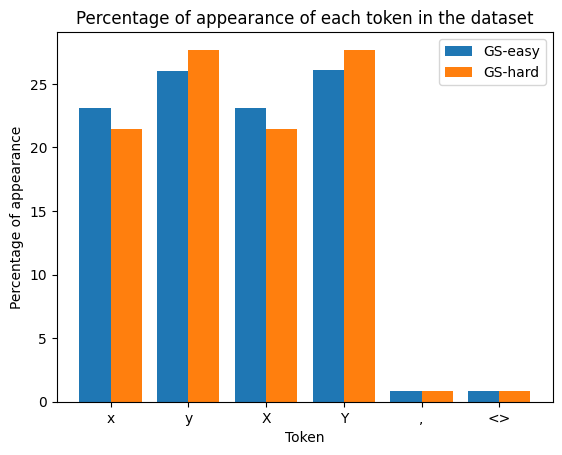
\includegraphics[scale=0.6]{fig/tokens_hist.png}
	\caption{Percentage of appearance of each token in the solved/unsolved datasets.}
	\label{fig:tokens_hist}
\end{figure}

\begin{figure}
	\centering
	\begin{subfigure}[b]{\textwidth}
		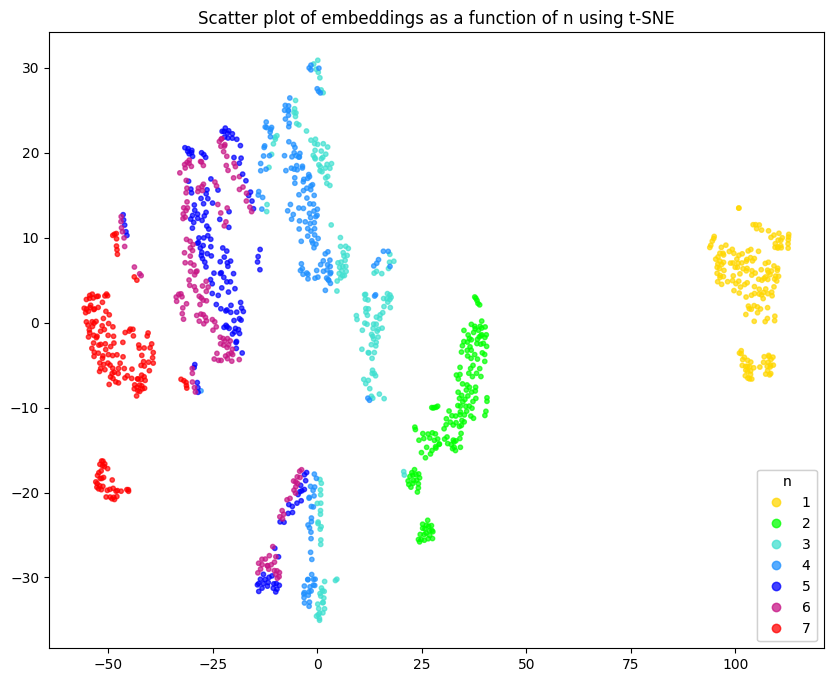
\includegraphics[width=\linewidth]{fig/embeddings_n.png}
		\caption{Scatter plot of embeddings as a function of $n$ using t-SNE}
		\label{fig:hist_vs_n}
	\end{subfigure}%
	%add desired spacing between images, e. g. ~, \quad, \qquad etc.
	%(or a blank line to force the subfigure onto a new line)

	\begin{subfigure}[b]{\textwidth}
		\centering
		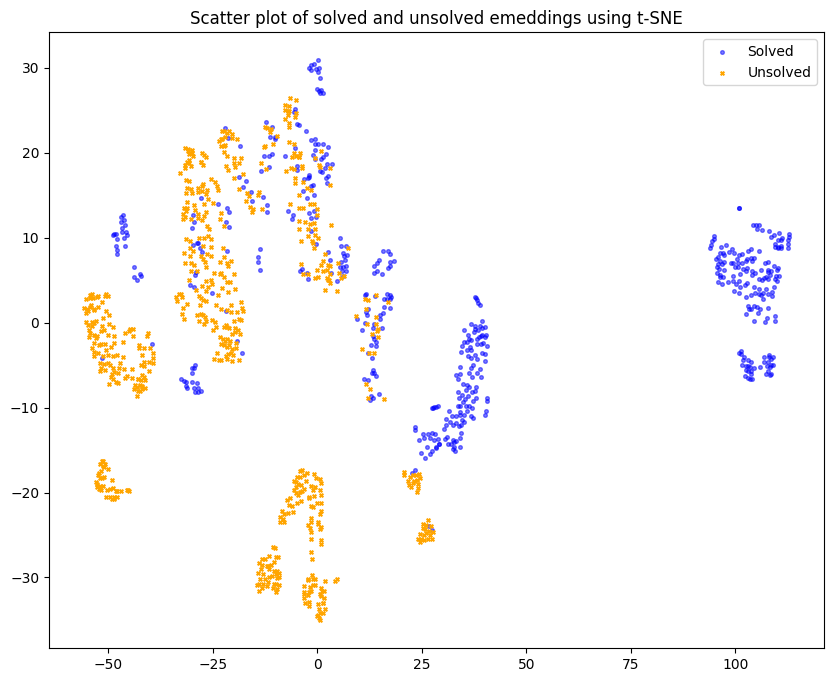
\includegraphics[width=\linewidth]{fig/embeddings_easy_vs_hard.png}
		\caption{Scatter plot of BFS-easy and BFS-hard examples using t-SNE}
		\label{fig:hist_vs_length}
	\end{subfigure}
	\caption{Projection of embeddings to a plane using t-SNE with cosine similarities}\label{fig:embeddings_tsne}
\end{figure}


\fixme{Is one way to interpret this result that the application of  BFS moves takes us far away from the initial presentation, but it still remembers which presentations should be hard vs easy?}
